\documentclass[10pt,a4paper,twocolumn]{article}

% Page layout
\setlength{\parindent}{.5cm}
\setlength{\columnsep}{.5cm}
\usepackage[left=2cm,right=2cm,top=2cm,bottom=2cm]{geometry}

% Encodings, characters, and typesetting
\usepackage[utf8]{inputenc}
\usepackage[T1]{fontenc}
\usepackage[english]{babel}
\usepackage{newtxtext,newtxmath} % access Times New Roman
\usepackage{microtype} % prettifies typesetting and prevents some overfulls

% Citation/reference management
\usepackage[citestyle=numeric-comp,bibstyle=numeric-comp,sorting=none,url=false,doi=false,useprefix=true,uniquename=false,uniquelist=false,giveninits=true,maxnames=2,natbib=true,backend=biber,]{biblatex}
\usepackage{csquotes} % prevents some warnings
\addbibresource{references.bib}
\renewbibmacro{in:}{}
\renewcommand{\bibopenparen}{\addcomma\addspace}
\renewcommand{\bibcloseparen}{\addperiod}
\DeclareFieldFormat[article,inbook,incollection,inproceedings,book,misc,unpublished]{title}{#1\isdot}
\DeclareNameAlias{default}{family-given}
% I have no clue why this works https://tex.stackexchange.com/a/352754
\DeclareNameFormat{author}{%
    \ifnumequal{\value{uniquename}}{0}
    {\usebibmacro{name:family}
       {\namepartfamily}
       {\namepartgiven}
       {\namepartprefix}
       {\namepartsuffix}}
    {\usebibmacro{name:family-given}
       {\namepartfamily}
       {\namepartgiven}
       {\namepartprefix}
       {\namepartsuffix}}%
    \usebibmacro{name:andothers}}


% Use comma and space between units
\renewcommand*{\newunitpunct}{\addcomma\space}
\AtEveryBibitem{%
  \clearfield{volume}%
  \clearfield{number}%
  \clearfield{pages}%
}

% Graphics/figures/tables
\usepackage{makecell}
\usepackage{booktabs}
\usepackage{graphicx}
\usepackage{subcaption}
\graphicspath{{./figures/}}
% \usepackage{makecell}
% \renewcommand\cellalign{lt}
\usepackage[font=small,labelfont=bf,labelsep=period,singlelinecheck=false]{caption}

\usepackage{siunitx}
\sisetup{group-digits=integer,group-separator={,},group-minimum-digits={3}}
%% see this important post about interaction between datatools and siunitx https://tex.stackexchange.com/a/23460


% Load data.
\usepackage{datatool}
\DTLsettabseparator

\DTLloaddb{totals}{data/describe-totalcounts.tsv}
\DTLloaddb{toptags}{data/describe-toptags.tsv}
\DTLloaddb{topcategories}{data/describe-topcategories.tsv}
\DTLloaddb{demop}{data/describe-demographics_provided.tsv}
\DTLloaddb{clf}{data/validate-classifier_avg.tsv}
\DTLloaddb{liwcstats}{data/validate-liwc_scores-stats.tsv}

\DTLassignfirstmatch{totals}{total}{posts}{\totalposts=count}
\DTLassignfirstmatch{totals}{total}{users}{\totalusers=count}

\DTLassignfirstmatch{demop}{demographic_variable}{gender}{\ngender=n_reported,\pctgender=pct_reported}
\DTLassignfirstmatch{demop}{demographic_variable}{age}{\nage=n_reported,\pctage=pct_reported}
\DTLassignfirstmatch{demop}{demographic_variable}{country}{\ncountry=n_reported,\pctcountry=pct_reported}
\DTLassignfirstmatch{demop}{demographic_variable}{gender+age+country}{\nall=n_reported,\pctall=pct_reported}

\DTLassignfirstmatch{clf}{scorer}{accuracy}{\clfaccm=CV mean,\clfaccsd=CV std}
\DTLassignfirstmatch{clf}{scorer}{f1}{\clffonem=CV mean,\clffonesd=CV std}

\DTLassignfirstmatch{liwcstats}{category}{insight}{\insightW=W-val,\insightP=p-val,\insightD=cohen-d,\insightCLES=CLES}
\DTLassignfirstmatch{liwcstats}{category}{agency}{\agencyW=W-val,\agencyP=p-val,\agencyD=cohen-d,\agencyCLES=CLES}
% \xDTLassignfirstmatch{liwcstats}{category}{agency}{\agencyW=W-val,\agencyP=p-val}

%%%%%%%%%% Unused but useful for other times.
% \usepackage{indentfirst} % indents first paragraphs of sections, following headings
% \usepackage{endfloat} % kick all floats to the end, useful while drafting


% Title page info
\title{\bf A large corpus of lucid and non-lucid dream reports}
\author{Remington Mallett \\
  Department of Psychology \\
  Northwestern University \\
  \texttt{mallett.remy@gmail.com}
  \and
  Ashwini Ashokkumar \\
  Department of Psychology \\
  Stanford University
}
\date{}



%%%%%%%%%%%%%%%%%%%%%%%%%%%%%%%%%%%%%%%%%%%  DOCUMENT STARTS
\begin{document}

\maketitle

%%%%% Uncomment to print column width in Points (pt), 1/72.27 of an inch.
% The column width is: \the\columnwidth



%%%%%%%%%%%%%%%%%%%%%%%%%%%%%%%%%%%% Abstract
\section*{Abstract}
All varieties of dreaming remain a mystery. Lucid dreams in particular -- those characterized by awareness of the dream -- are notoriously difficult to study. Their scarce prevalence and resistance to artificial induction make it difficult to obtain a sizeable corpus of lucid dream reports. The consequent lack of clarity around lucid dream phenomenology has left the many purported applications of lucidity under-realized. Here, a large dataset of 10k lucid and 25k non-lucid dream reports from 5k contributors is curated, described, and validated for future lucid and non-lucid dream studies. Ten years of publicly available dream reports were scraped from an online forum where users share anonymous dream journals. Importantly, users could optionally identify their dream as lucid or non-lucid, offering a user-generated labeling system for research. After characterizing the dataset with descriptive statistics and visualizations, these lucidity labels are validated by showing that language patterns in lucid-labeled reports are consistent with known characteristics of lucid dreams. While the entire corpus has broad value for dream studies, the labeled subset is particularly powerful for new discoveries in lucid dream research.

\bigskip
\noindent {\bf Keywords:} sleep, dreaming, big data, text mining, nlp



%%%%%%%%%%%%%%%%%%%%%%%%%%%%%%%%%%%%%%%%%%%%%%%%% Intro
\section{Introduction}
\label{sec:introduction}

Lucid dreams are those that include awareness of the dream while dreaming \cite{baird2019}. They are often associated with control over dream content \cite{lemyre2020}, which is commonly used to experience fun and impossible behaviors while sleeping \cite{stumbrys2014}. Despite early promise of lucid dreaming applications in therapy \cite{demacedo2019} and research \cite{konkoly2021}, the variety and detail of what it is \emph{like} to be lucid while dreaming is still unclear \cite{mallett2021}. This conflict, of application endorsement on the one hand and limited scientific understanding on the other, has raised concerns about whether some lucid dreaming practices are being implemented too soon \cite{vallat2019,soffer2020}. Are we ``leaping before we look'' with respect to lucid dreaming applications?

\par
Without sufficient data on lucid dreams, it is difficult to ``look'' at all. Quantitative studies of lucid dreaming are often hindered by low sample sizes. Lucid dream occurrence is relatively rare in nature \cite{saunders2016} and they are difficult to induce reliably \cite{stumbrys2012}, making it difficult to accumulate enough data for strong conclusions. To overcome this limitation, I looked to a rising trend in computational social science, the use of digital trace data to accumulate large and naturalistic datasets \cite{lazer2021}.

\par
The ubiquity of digital media in daily life has provided a major data source for psychologists \cite{lazer2021,shah2015,kern2016,gosling2015,rafaeli2019,heng2018}. The ability to view online human behavior en masse has been hailed as social science's first true ``telescope'' \cite{jungherr2017}. Datasets curated from popular social media sites (e.g., Twitter, Reddit) are not only large, but also free from experimenter intervention or influence, a major methodological concern in psychological research that dream studies are not immune to \cite{picard2021, schredl2002}. Thus, dream science could benefit as well from the use of digital trace data \cite{bulkeley2017} and in recent years has \cite{sanz2018, niederhoffer2017, elce2021}. While dream reports are harder to extract from mainstream social media sites, it is common practice for researchers to scrape specialized data from targeted forums \cite{speckmann2021}. To build a large corpus of (lucid) dreams, we scraped DreamViews\footnote{https://www.dreamviews.com}, an online lucid dreaming journal active since 2010.

\par
The current paper presents the collection, characterization, and validation of this dataset. First, the process of data collection, cleaning, and user-generated label extraction (lucid, non-lucid, and nightmare) is described. Second, the general size and details of the final corpus are presented. Last, natural language processing tools \cite{hirschberg2015,elce2021} are used to show that the lucid, non-lucid, and nightmare labels provided by users have criterion validity. That is, the content of lucid dreams and nightmares in the corpus show expected properties based on prior literature \cite{voss2013,paquet2020}. This validation justifies the use of these labels for future studies. Code used to generate and analyze the entire corpus of $\sim$55k dream reports (10k lucid, 25k non-lucid, 2k nightmare) is freely available\footnote{https://github.com/remrama/dreamviews\_ds}.



%%%%%%%%%%%%%%%%%%%%%%%%%%%%%%%%%%%%%%%%%%%%%%%%%%%%% Methods
\section{Methods}
\label{sec:methods}

\subsection{Data source}
\label{sec:data-source}

DreamViews is a public and anonymous online forum dedicated to lucid dreaming. In addition to the discussion threads and user profiles typical of most forums, users can also share a public dream journal. An example dream journal entry is offered in Figure~\ref{fig:journal-entry}. Each journal entry includes a dream report (hereafter, ``post''), a title, and the option to attach ``category'' and ``tag'' labels that help identify features of the dream.

\par
The DreamViews label system plays a major role in the curation of this dataset because it allows for the isolation of certain types of dreams for study and comparison (similar to its online function of viewing dreams by label). When a user adds one or more category labels to their dream journal entry, their options are restricted to a small subset of terms provided by DreamViews (e.g., \emph{lucid}, \emph{non-lucid}, \emph{memorable}). In contrast, tag labels are unconstrained and thus consist of far variety across participants (e.g., a barista who dreams about work a lot might be the only user with a \emph{coffee} tag), as well as varied spellings (e.g., \emph{non-lucid}, \emph{nonlucid}, and \emph{nld}). Only category labels were used to derive lucidity and nightmare labels, whereas future work might take advantage of the varied tag labels available in this dataset.


%%%%%%%%%%%%%%%%%%%%%%%%%%%%%%% START figures/tables

\begin{figure}[t]
    \centering
    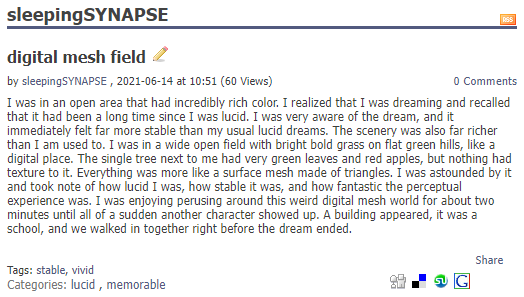
\includegraphics[width=\columnwidth]{journal_entry.png}
    \caption{Example DreamViews dream journal entry. The Categories labeling system, seen at the bottom, was used to extract labels for the corpus. This entry is from the author's journal.}
    \label{fig:journal-entry}
\end{figure}

%%%%%%%%%%%%%%%%%%%%%%%%%%%%%%% END figures/tables


\subsection{Data collection}
\label{sec:data-collection}

All public DreamViews dream journal entries between years 2010 and 2020 (inclusive) were scraped \cite{speckmann2021,li2019,landers2016} using custom code on December 12\textsuperscript{th}, 2021, starting from the dream journal homepage\footnote{https://www.dreamviews.com/blogs} and crawling over all ``view all'' pages. Raw HTML was parsed to extract each journal entry's post (i.e., dream report text), title, tags, categories, timestamp, and user. The public profiles of dream journal users were scraped for self-reported demographic information (usernames were replaced with a random identifier). All text was converted to ASCII\footnote{https://github.com/avian2/unidecode}.


\subsection{Text processing}
\label{sec:text-preprocessing}

\smallskip
\noindent
\textbf{Cleaning.}
Text was minimally cleaned with the aims of standardization, removing non-dream content, and removing potentially private or identifying information. Consecutive whitespaces were replaced with a single space, ampersands were replaced with text (\texttt{and}), common contractions were expanded, and sequences of four or more repeated characters \cite{gray2020} were reduced to a single character. A regex pattern was used to replace emails and URLs with \texttt{[[URL]]}, and named entity recognition was used to identify and replace names with \texttt{[[NAME]]}. Named entity recognition was implemented using \emph{spaCy}\footnote{https://spacy.io}, which typically outperforms related software \cite{shelar2020,jiang2016}. Visual inspection revealed non-dream character sequences that were frequent and reliable across multiple posts, and these were removed using custom regex patterns (see online code for specifics).

\smallskip
\noindent
\textbf{Lemmatization.}
Cleaned posts were further reduced and lemmatized to produce text more suitable for most language analyses while also providing an additional precautionary layer of privacy protection. Cleaned text was tokenized using \emph{spaCy}. A token was removed if it contained a non-alphabetic character, was shorter than three characters, was a stop word or proper noun (as identified by \emph{spaCy}), or had a low probability of being in \emph{spaCy}'s vocabulary (to estimate mispellings or otherwise uncommon character sequences). All retained tokens were lemmatized with \emph{spaCy} and lowercased, and token order was shuffled.


\subsection{Data exclusion}
\label{sec:data-exclusion}

Posts were removed if estimated as non-English\footnote{https://github.com/Mimino666/langdetect}, or containing $<$50 or $>$1k words (counted from cleaned text). In an effort to reduce single-user biases within the corpus, only the first 1k posts from a given user (that passed prior criteria) were kept. Visual inspection revealed, on minor occasion, systematic features of posts that indicated there was no dream content present (see online code for specifics). Such posts were removed.


\subsection{User-generated labels}
\label{sec:automated-labeling}

The category labels attached to journal entries were used to identify the lucidity level of a post (\emph{lucid} or \emph{non-lucid}) and if the post was a \emph{nightmare} (see Figure~\ref{fig:journal-entry} and Section~\ref{sec:data-source}). For each journal entry where the user attached category labels, they were searched for relevant terms. To identify lucidity, terms ``lucid'' and ``non-lucid'' were searched; a post was identified as \emph{unspecified} if neither label was provided, \emph{ambiguous} if both labels were provided, and either \emph{lucid} or \emph{non-lucid} if one was provided without the other. Similarly, the term ``nightmare'' was searched, and a post was identified as a \emph{nightmare} if the term was present and \emph{non-nightmare} otherwise.


%%%%%%%%%%%%%%%%%%%%%%%%%%%%%%% START figures/tables

\begin{table}[t]
    \caption{Description of datafiles.}
    \label{table:datafiles}
    \begin{subtable}[t]{.48\textwidth}
        \caption{Columns of \texttt{dreamviews-posts.tsv}.}
        \label{table:datafile-posts}
        \small
        \begin{tabular}{rrl}
            \toprule
            column & dtype & value \\
            \midrule
            post\_id & str & unique randomized post identifier \\
            user\_id & str & unique randomized user identifier \\
            timestamp  & str & date and time of post (ISO 8601) \\
            nth\_post & int & user's nth post in dataset \\
            title & str & post title \\
            tags & str & tag labels of post \\
            categories & str & category labels of post \\
            % lucidity & str & \makecell{derived lucid label  \\ \texttt{lucid}, \texttt{nonlucid}, \\ \texttt{unspecified}, or \texttt{ambiguous}} \\
            % nightmare & bool & \makecell{\texttt{True} if post was identified \\ as a nightmare else \texttt{False}} \\
            lucidity & str & derived lucid label \\
            nightmare & bool & derived nightmare label \\
            wordcount & int & number of words in post \\
            post\_clean & str & cleaned post \\
            post\_lemmas & str & lemmatized post \\
            \bottomrule
        \end{tabular}
    \end{subtable}

    \bigskip
    \begin{subtable}[t]{.48\textwidth}
        \caption{Columns of \texttt{dreamviews-users.tsv}.}
        \label{table:datafile-users}
        \small
        \begin{tabular}{rrl}
            \toprule
            column & dtype & value \\
            \midrule
            user\_id & str & unique randomized user identifier \\
            gender  & str & reported gender \\
            age     & int & reported age \\
            country & str & reported country (ISO 3166-1 alpha-3) \\
            \bottomrule
        \end{tabular}
    \end{subtable}
\end{table}

\begin{figure*}[t]
    \centering
    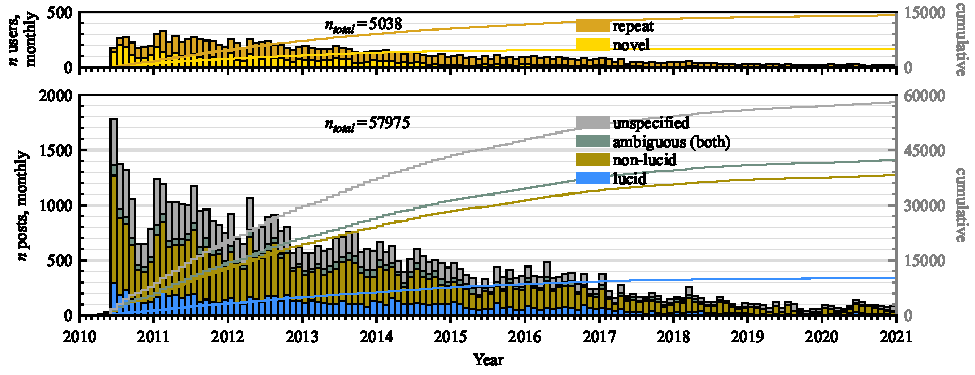
\includegraphics{describe-timecourse.pdf}
    \caption{Total corpus size. Left axis values correspond to bars and right axis values correspond to cumulative distribution lines. Note that the final cumulative distributions endpoints provide a rough visualization of total corpus counts. The top panel shows the number of unique users that posted each month, where repeat/gold users are those that also posted in a prior month. The bottom panel shows the amount of unique posts each month, where colors indicate the lucidity label of posts. Note that the popular lucid dreaming film \emph{Inception} saw releases in July and December of 2010.}
    \label{fig:timecourse}
\end{figure*}

\begin{figure}[t]
    \centering
    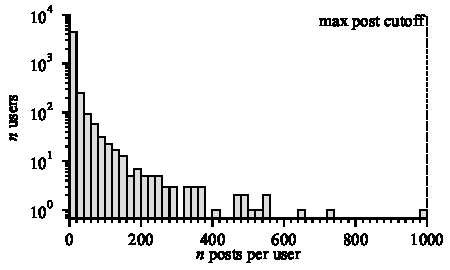
\includegraphics{describe-usercount.pdf}
    \caption{Number of posts per user.}
    \label{fig:usercount}
\end{figure}

\begin{figure*}
    \begin{subfigure}[t]{0.3\textwidth}
        \centering
        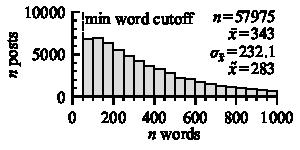
\includegraphics{describe-wordcount_perpost.pdf}
        \caption{Word count per post. This histogram treats each dream report with equal weight, not accounting for repeated measurements within users.}
        \label{fig:wordcount1}
    \end{subfigure}
    \hfill
    \begin{subfigure}[t]{0.3\textwidth}
        \centering
        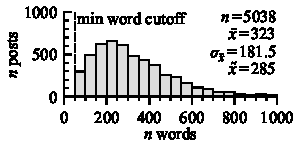
\includegraphics{describe-wordcount_peruser.pdf}
        \caption{Word count per post, per user. Data in this histogram was first averaged to get a single word count per post for each individual user.}
        \label{fig:wordcount2}
    \end{subfigure}
    \hfill
    \begin{subfigure}[t]{0.3\textwidth}
        \centering
        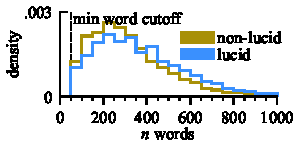
\includegraphics{describe-wordcount_lucidity.pdf}
        \caption{Word count per post, per user, by lucidity. Data in this histogram was first averaged to get a single word count per post for each individual user. Then lucid and non-lucid posts were plotted separately. Lucid dream reports contained a higher word count than non-lucid dream reports.}
        \label{fig:wordcount3}
    \end{subfigure}
    \caption{Number of words per dream report. $n$: sample size, $\bar{x}$: mean, $\sigma_{\bar{x}}$: standard deviation, $\tilde{x}$: median}
    \label{fig:wordcount}
\end{figure*}

\newcolumntype{L}{>{\raggedright\arraybackslash}X}
\newcolumntype{R}{>{\raggedleft\arraybackslash}X}

\begin{table}[t]
    \caption{Top category and tag labels.}
    \label{table:toplabels}
    \begin{subtable}[t]{.25\textwidth}
        \caption{Top category labels.}
        \label{table:topcategories}
        \small
        \begin{tabular}{rp{1cm}}
            \toprule
            \bfseries category & \bfseries \makecell[rt]{n posts\\users}
            \DTLforeach*{topcategories}{\cat=category, \nposts=n_posts, \nusers=n_users}{
                \DTLiffirstrow{\\\midrule}
                \\\cat & \makecell[rt]{\num{\nposts}\\\num{\nusers}}
                \ifthenelse{\value{DTLrowi}=10}{\dtlbreak}{}
            }
            \\\bottomrule
        \end{tabular}
    \end{subtable}%
    \hfill
    \begin{subtable}[t]{.2\textwidth}
        \caption{Top tag labels.}
        \label{table:toptags}
        \small
        % \begin{tabular}{@{} rp{1cm} @{}}
        \begin{tabular}{rp{1cm}}
            \toprule
            \bfseries tag & \bfseries \makecell[rt]{n posts\\users}
            \DTLforeach*{toptags}{\tag=tag, \nposts=n_posts, \nusers=n_users}{
                \DTLiffirstrow{\\\midrule}
                \\\tag & \makecell[rt]{\num{\nposts}\\\num{\nusers}}
                \ifthenelse{\value{DTLrowi}=10}{\dtlbreak}{}
            }
            \\\bottomrule
        \end{tabular}
    \end{subtable}
\end{table}

\begin{figure}[t]
    \centering
    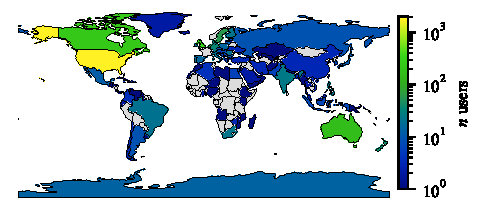
\includegraphics{describe-demographics_location.pdf}
    \caption{Reported user locations.}
    \label{fig:demographics-location}
\end{figure}

\begin{figure}[t]
    \centering
    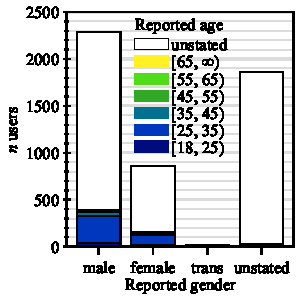
\includegraphics{describe-demographics_agegender.pdf}
    \caption{Reported user age and gender.}
    \label{fig:demographics-agegender}
\end{figure}

%%%%%%%%%%%%%%%%%%%%%%%%%%%%%%% END figures/tables


\subsection{Availability of materials}
\label{sec:availability}

All code used to generate and analyze the current corpus is publicly available. The final corpus is available on Zenodo and abides by the modern FAIR principles of data management and stewardship \cite{wilkinson2016}. The two tab-separated value files that make up the corpus are ASCII-encoded with missing values as ``NA'' (detailed in Table~\ref{table:datafiles}).
% The publicly released and doi-stamped dataset released with this paper consists of \emph{lemmatized} posts of the entire corpus (see Section~\ref{sec:data-files}). Full \emph{cleaned} posts, post attributes (e.g., title), and demographic information are available upon request or by utilizing the code referenced in the previous paragraph. For reasoning, see Sections~\ref{ethical-considerations} and~\ref{sec:extended-ethics}. The public release of this dataset abides by the modern FAIR principles of data management and stewardship \cite{wilkinson2016fair}. The data are Findable through a persistent doi, Accessible through multiple formats (doi, self-generation, request), Interoperable in that the \texttt{tsv} file format is universal and readable by most modern software, and Reusable in that it retains a CC license and this current paper is dedicated to describing its features and value. As for the subsetted data release, slight adjustments and re-considerations from the original FAIR proposal are warranted with digital trace data \cite{boeckhout2018fair, mons2017cloudy}.


\subsection{Ethical considerations}
\label{sec:ethical-considerations}

This research was deemed exempt from IRB approval by the Northwestern IRB Review Board. Best-practice community standards were followed at all stages of work \cite{rivers2014,zook2017,franzke2020}, such as making no attempt to gather additional information not already public, making no attempt to de-anonymize users, and being transparent with the data collection method. This corpus is derived exclusively from publicly available data, and no Terms of Service or electronic prevention methods were breached during data collection \cite{boegershausen2021,krotov2018,krotov2020,gold2017}.
% The ethics of social media or digital trace data is an ongoing debate \cite{zwitter2014big, ferretti2021ethics, metcalf2016human, lazer2020computational, lazer2021, shah2015}, which can be loosely split into the ethics of analyzing versus sharing such data. In the analysis of such data and presenting it in aggregated form... Due to situational nuance, I opted to take a mixed approach of precaution an openness \cite{boeckhout2018fair, weller2016manifesto, meyer2018practical, towse2021opening}. As described in Sections~\ref{sec:data-collection} and~\ref{sec:text-preprocessing}, additional steps were taken to ensure potential efforts of de-anonymization, including the removal of any non-essential data (e.g., entry titles, usernames), removal of any URLs, emails, names, and proper nouns, heavy text processing (e.g., lemmatization), and the shuffling of words to prevent any sensible sentence structure or actual reading of the text. See Section~\ref{sec:extended-ethics} for a lengthy discussion on this topic.



%%%%%%%%%%%%%%%%%%%%%%%%%%%%%%%%%%%%%%%%%%%%%%%%%%%%%%%%%%%%%%%%%%%%%%
\section{Data description}
\label{sec:description}

% The released dataset consists of a single file, \texttt{dreamviews-posts-superanon.tsv}, with all the same rows/posts but slightly reduced column information (see Section~\ref{sec:availability}).
% The final released dataset consists of a single tab-separated value file, \texttt{dreamviews-posts-superanon.tsv}, with \texttt{utf-8} encoding. Tab-separated values files are similar to comma-separated files but cause less complications universally and with text data (here, all post tabs were replaced with single spaces, see Section~\ref{text-preprocessing}). Missing values were coded as \texttt{NA}. The file consists of five columns, explained in Table~\ref{table:posts-columns}.

\subsection{General characterization}
\label{sec:general-characterization}

The final corpus contains \num{\totalposts} dream reports from \num{\totalusers} unique users. Post frequency is presented in the bottom panel of Figure~\ref{fig:timecourse}. Post frequency steadily declined over time, reducing to very little activity in recent years. Many users contributed multiple posts to the corpus, as indicated in the top panel of Figure~\ref{fig:timecourse} and in Figure~\ref{fig:usercount}. The most common category and tag labels are presented in Table~\ref{table:toplabels}.


\subsection{Demographics}
\label{sec:demographics}

A variable amount of demographic information was self-reported in the public user profiles. Reported age and gender are presented in Figure~\ref{fig:demographics-agegender} and reported location in Figure~\ref{fig:demographics-location}. Of users in the final corpus, \num{\ngender} (\num{\pctgender}\%) provided a gender, \num{\nage} (\num{\pctage}\%) reported an age, \num{\ncountry} (\num{\pctcountry}\%) reported a location, \num{\nall} (\num{\pctall}\%) users reported all three. Profiles suggest that users lean towards males in early adulthood from the United States. Non-English posts were removed before aggregation, which might have influenced location results.


\subsection{Word count}
\label{sec:word-count}

Word count is a critical consideration when quantifying text and especially important when evaluating dream reports \cite{urbina1981,schredl1999,schredl2011,rover2017,rosenlicht1994,antrobus1983}. Counts are presented in Figure~\ref{fig:wordcount} as the number of words per cleaned post rather than lemmatized post (see Section~\ref{sec:text-preprocessing}). Word counts are presented in a few ways, emphasizing the importance of accounting for user dependencies and showing the difference between lucid and non-lucid posts.

% \begin{table}[t]
%     \caption{Word/lemma summary statistics for lucid and non-lucid posts. Counts were first averaged within user.}
%     \label{table:wordcount}
%     \small
%     \begin{tabular}{rrrrr}
%         \toprule
%             {} & \multicolumn{2}{l}{word} & \multicolumn{2}{l}{lemma} \\
%             {} & non-lucid & lucid & non-lucid & lucid \\
%         \midrule
%             mean   &       318 &   366 &       114 &   132 \\
%             std    &       178 &   197 &        65 &    72 \\
%             min    &        50 &    50 &        15 &    13 \\
%             median &       284 &   334 &       103 &   121 \\
%             max    &      1000 &   997 &       417 &   379 \\
%         \bottomrule
%     \end{tabular}
% \end{table}


%%%%%%%%%%%%%%%%%%%%%%%%%%%%%%% START figures/tables

\begin{figure}[t]
        \centering
        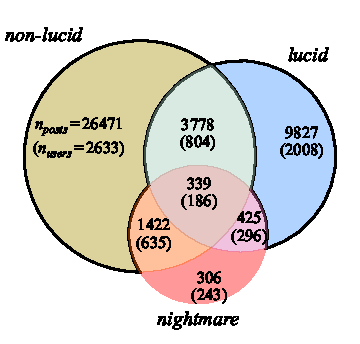
\includegraphics{describe-categorycounts.pdf}
        \caption{User-generated label frequencies, per post and per user. Within each section, the top number represents the number of posts and the bottom number represents the number of unique users that contribute to the post count. Non-lucid labels occur the most frequently, lucid labels second, and nightmare labels least. Venn sets are sized proportionally to user-normalized post frequencies.}
        \label{fig:categorycounts}
\end{figure}

\begin{figure}[t]
        \centering
        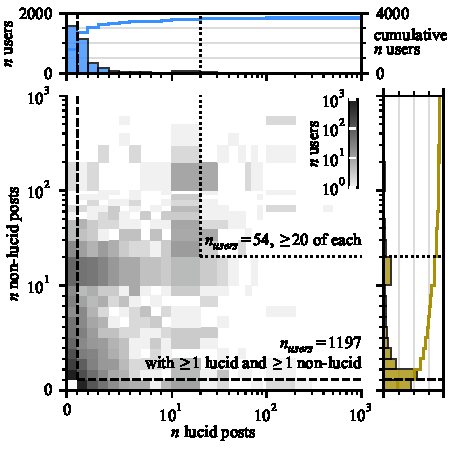
\includegraphics{describe-categorypairs.pdf}
        \caption{The frequency of users contributing lucid and non-lucid posts. The center panel highlights the number of users at each lucid and non-lucid post frequency. The dashed lines close a box around all post frequencies that include $>$0 lucid and $>$0 non-lucid, and the inner text provides the total number of users this is true for. The dotted lines close a box around all post frequencies that includes  $>$20 lucid and $>$20 non-lucid, motivated by the finding that 20 dream reports provides a stable estimate of dream content within individuals \cite{schredl1998}.
        Distributions in the marginal panels indicate the raw and cumulative number of users who contribute to either lucid or non-lucid post frequencies.}
        \label{fig:categorypairs}
\end{figure}

%%%%%%%%%%%%%%%%%%%%%%%%%%%%%%% END figures/tables


\subsection{Lucidity label frequency}
\label{sec:lucidity-label-frequency}

Because the user-generated labeling of lucidity was not available for every post, it is important to understand what subset of the data \emph{does} include labels. The bottom panel of Figure~\ref{fig:timecourse} (cumulative distributions) provides a rough visualization of absolute and relative label frequencies. What that figure does not reveal is how many users contribute to each label (e.g., does one user contribute all the lucid posts?). Figure~\ref{fig:categorycounts} conveys this information, and also shows the overlap amongst labels more explicitly. This diagram shows there are roughly 14k posts labeled as lucid, with $\sim$4k of them also labeled as non-lucid and $\sim$500 of them also labeled as a nightmare. The overlap of lucid and non-lucid posts with nightmare labels shows the amount of data available for future analyses comparing lucid nightmares agains non-lucid nightmares. Another important consideration when choosing an analysis is the number of users contributing \emph{both} a lucid and a non-lucid post, as well as the total number of lucid and non-lucid posts each individual user contributes. These factors, presented in Figure~\ref{fig:categorypairs}, are important when considering statistical power and the reliability of dream reports \cite{schredl1998}. The center shading represents the number of users who contribute each combination of lucid and non-lucid posts. The larger dashed line inset highlights the users who contributed one or more of each type of dream report (i.e., lucid and non-lucid). The smaller dashed subset indicates the same but for users with 20 or more of each post type. This visualization is useful in determining the amount of data for within-subjects lucid and non-lucid dream report comparisons. The marginal distributions isolate each dream type, showing the amount of users who contribute at each frequency level for lucid and non-lucid posts.



%%%%%%%%%%%%%%%%%%%%%%%%%%%%%%%%%%%%%%%%%%%%%%%%%%%%%%%%%%%%%%%%%%%%%%
\section{Validation}
\label{sec:validation}

The purpose of this section is to validate the user-generated labeling process described throughout prior sections. Before the labels can be used to make novel observations, they first need to be shown that they accurately represent the known features of the dream type they are supposed to represent (i.e., criterion validity). Posts identified as lucid should ``look'' lucid \cite{stumbrys2014,motarolim2013,bulkeley2018,voss2013,mallett2021}, and posts identified as a nightmare should look like nightmares \cite{standards2010,bulkeley2018}.

\par
The validation steps proceed with increasing specificity in the following order. First, Section~\ref{sec:classifier} uses a classification approach to evaluate whether the language of lucid and non-lucid posts are different in a general sense. Next, Section~\ref{sec:wordshift} uses frequency-weighted measures to visualize word-level differences between lucid and non-lucid posts and assess their alignment with known lucid features (similarly for nightmares). Last, Section~\ref{sec:liwc} tests specific hypotheses about which psychological constructs appear more in lucid posts (namely insight and agency).


\subsection{General distinction}
\label{sec:classifier}

This goal of this analysis was to determine whether lucid and non-lucid posts have different language use. A classifier was trained on word frequencies to identify a post as lucid or non-lucid.

\smallskip
\noindent
\textbf{Methods.} Classification was implemented using \emph{scikit-learn}\footnote{https://scikit-learn.org} \cite{pedregosa2011}. Each lemmatized post was transformed into a word-frequency vector. Very frequent (appearing in $>$75\% of posts) or infrequent (appearing in $<$100 posts) words were removed, after which the top 5k words were kept as features. A linear support vector machine classifier was used with a regularization parameter of 1. To avoid user-specific biases, a single post per user was randomly selected (irrespective of lucidity label) and then the more frequent class was downsampled to match the size of the smaller class. A stratified-shuffle-split cross-validation scheme was implemented, with the classifier trained on 70\% of posts and tested on the other 30\% at each of 5 folds. Note that performance was not optimized in any way (e.g., with hyperparameter tuning).

\smallskip
\noindent
\textbf{Results.}
Lucid and non-lucid posts were easily distinguishable under this ``out-of-the-box'' classification model. Across cross-validation folds, classifier accuracy was \num[round-mode=places,round-precision=2]{\clfaccm}$\pm$\num[round-mode=places,round-precision=2]{\clfaccsd}\% (M$\pm$SD, chance 50\%). Similar results were obtained with F1-score (\num[round-mode=places,round-precision=2]{\clffonem}$\pm$\num[round-mode=places,round-precision=2]{\clffonesd}\%). This suggests that there are indeed meaningful language differences between the lucid and non-lucid posts in this corpus. Future work might optimize the present classification model and test its generalizability to novel and lab-based lucid dream reports.


%%%%%%%%%%%%%%%%%%%%%%%%%%%%%%% START figures/tables

\begin{figure}[t]
    \centering
    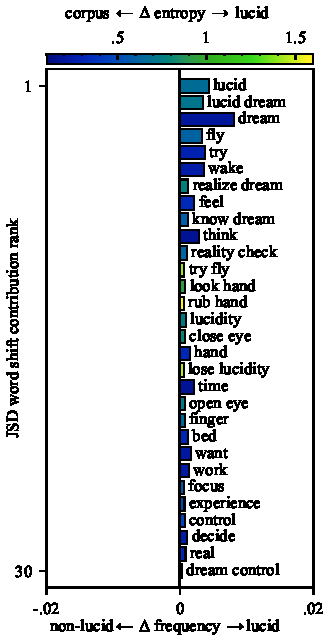
\includegraphics{validate-wordshift_jsd-myplot.pdf}
    \caption{Lucidity JSD word shift. Words and phrases that most distinguish user-labeled lucid and non-lucid dream reports are consistent with known lucidity characteristics. These results offer concurrent validity for user-generated lucidity labels.}
    \label{fig:wordshift-jsd}
\end{figure}

\begin{figure}[t]
    \centering
    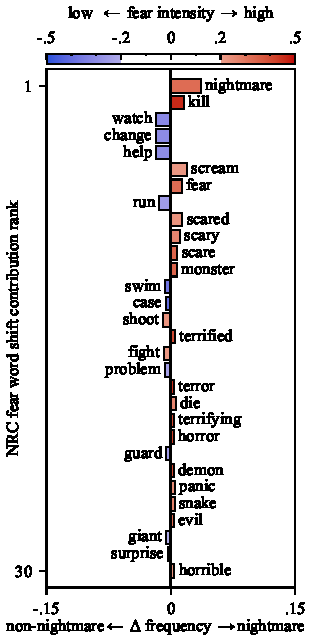
\includegraphics{validate-wordshift_fear-myplot.pdf}
    \caption{Nightmare fear word shift. Words and phrases that most distinguish user-labeled nightmares from all other dream reports are consistent with known nightmare characteristics. These results offer concurrent validity for user-generated nightmare labels.}
    \label{fig:wordshift-fear}
\end{figure}

\begin{figure*}[t]
    \begin{subfigure}[t]{0.3\textwidth}
        \centering
        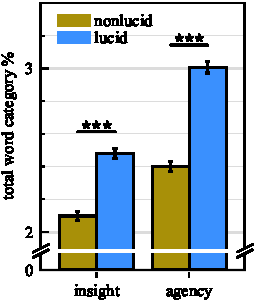
\includegraphics{validate-liwc_scores-plot.pdf}
        \caption{LIWC insight and agency language differences between user-labeled lucid and non-lucid dream reports. Lucid dream reports contained higher rates of both insight and agency than non-lucid dream reports. Error bars represent SEM, ***$p<.001$}
        \label{fig:liwc-categories}
    \end{subfigure}
    \hfill
    \begin{subfigure}[t]{0.3\textwidth}
        \centering
        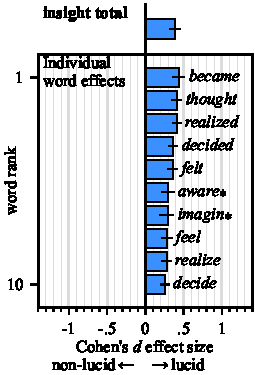
\includegraphics{validate-liwc_wordscores_insight-plot.pdf}
        \caption{Word-level differences of insight language between user-labeled lucid and non-lucid dream reports. Insight was quantified as the percentage of words from LIWC's insight dictionary in each dream report. Error bars represent bootstrapped 95\% confidence intervals. Asterisks indicate wildcard patterns.}
        \label{fig:liwc-words-insight}
    \end{subfigure}
    \hfill
    \begin{subfigure}[t]{0.3\textwidth}
        \centering
        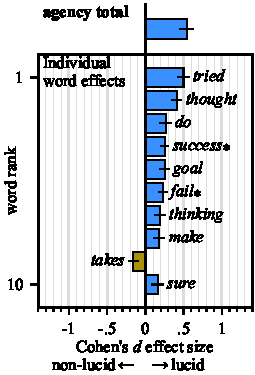
\includegraphics{validate-liwc_wordscores_agency-plot.pdf}
        \caption{Word-level differences of agency language between user-labeled lucid and non-lucid dream reports. Agency was quantified as the percentage of words from LIWC's agency dictionary in each dream report. Error bars represent bootstrapped 95\% confidence intervals. Asterisks indicate wildcard patterns.}
        \label{fig:liwc-words-agency}
    \end{subfigure}
    \caption{LIWC validation results. Dream reports labeled as lucid by the user contain a higher percentage of insight and agency dictionary words than those labeled as non-lucid dream reports. These results offer construct validity for the user-labeled dream reports.}
    \label{fig:liwc}
\end{figure*}

%%%%%%%%%%%%%%%%%%%%%%%%%%%%%%% END figures/tables



\subsection{Word-level differentiation}
\label{sec:wordshift}

The goal of this step was to validate labels by examining fine-grained differences between the language of posts and assess their consistency with predictable dream characteristics. Do lucid posts contain phrases common to lucid dream reports and culture, such as ``knew it was a dream'' and ``reality check?'' Do nightmare posts contain phrases that represent fear, such as ``scared'' and ``monster?'' These questions were answered using word shifts, a new approach to comparing texts that takes traditional word-frequency differences and adds context-specific weights \cite{gallagher2021}. Word shifts were used to identify the words (unigrams and bigrams) that contribute most to the separation between two texts (lucid vs. non-lucid, nightmare vs. non-nightmare), and the consistency of those words with prior literature was qualitatively assessed.

\smallskip
\noindent
\textbf{Methods.}
Word shift analyses were run on lemmatized posts using \emph{Shifterator}\footnote{https://github.com/ryanjgallagher/shifterator} \cite{gallagher2021} with common co-occuring unigrams first converted to bigrams using \emph{Gensim}\footnote{https://radimrehurek.com/gensim} \cite{rehurek2010}. A detailed presentation of word shift methods are available elsewhere \cite{gallagher2021}. The only additional step performed here was a normalization during initial calculation of word frequencies. Rather than summing word frequencies across all posts, user dependencies were accounted for by first dividing the word frequencies of each user by that user's number of posts (all within each corpus).

\par
To identify words that most distinguish lucid from non-lucid posts, frequency differences were weighted by a word's relative Jensen-Shannon divergence (JSD), a measure of entropy (i.e., rarity or ``surprisal'') \cite{lin1991}. Entropy has been shown to be useful in comparing texts, and was additionally chosen here based on the expectation that lucid posts would contain a higher frequency of words that are otherwise rare in other contexts. When identifying top words, the overall JSD word shift score (and thus rank) is determined by three factors: frequency difference between lucid and non-lucid posts, entropy differences between lucid and non-lucid posts, and entropy relative to the entire corpus.

\par
To identify words that most distinguish nightmare posts from non-nightmare (i.e., all other) posts, frequency differences were weighted by a word's fear-intensity score from the NRC Emotion Intensity Lexicon \cite{mohammed2018}, a crowdsourced and freely available\footnote{http://saifmohammad.com/WebPages/AffectIntensity.htm} set of ratings for a variety of emotions. The motivation to use fear-weighted frequency differences was based on the clear expectation that nightmare posts should contain a higher frequency of words associated with fear. Only words with a fear intensity rating outside of range \numrange{-.2}{.2} (full range \numrange{-.5}{.5})   were included in this analysis to reduce the influence of neutral words. When identifying top words, the overall fear word shift score (and thus rank) is determined by two factors: frequency difference between the two texts and the NRC fear intensity score.

\smallskip
\noindent
\textbf{Results.}
The JSD entropy word shift comparing lucid and non-lucid posts is presented in Figure~\ref{fig:wordshift-jsd}. Nearly all words that contribute to separating these texts are aligned with expected properties of lucid dream reports (face criterion validity). First, the word ``lucid'' appears in multiple phrases that distinguish lucid and non-lucid posts (all at a higher frequency in lucid posts). Second, words relating to cognitive effort or deliberate action -- such as ``think,'' ``try,'' ``control,'' and ``want'' -- are distinguishing words that appear more frequently in lucid than non-lucid posts. Third, ``fly'' appears in multiple phrases that are more frequent in lucid than non-lucid posts, and flying is one of the most commonly reported lucid actions \cite{stumbrys2014,motarolim2013,schadlich2012,barrett1991}. Fourth, many of the phrases that distinguish the corpora relate to lucid-dream-induction methods \cite{stumbrys2012}, including ``reality check,'' ``look hand,'' and ``rub hand.'' Fifth, distinguishing words such as ``feel'' and ``real'' are more frequent in lucid than non-lucid posts. These words might relate to an increased vividness in lucid dreams, as there are scattered reports that a subset of lucid dreams are particularly vivid \cite{redditpaper}.

\par
The fear intensity word shift comparing nightmare and non-nightmare (i.e., unlabeled) posts is presented in Figure~\ref{fig:wordshift-fear}. Nightmare posts have a clear bias towards intense fear words. Words that appear more frequently in nightmare posts are also higher in fear intensity, including ``kill,'' ``scream,'' ``monster,'' and ``panic.'' In contrast, words low on fear intensity like ``swim'' and ``case'' occur less frequently in nightmare posts. The few fear words that \emph{do} appear more in non-nightmare posts -- ``fight'' and ``shoot'' -- are lower in fear intensity and consistent with the high rates of daily activities in dream content (e.g., sports or social quarrels)~\cite{schredl2010}.


% \vfill % Temporary while it improves the current layout.


\subsection{Cognitive language markers}
\label{sec:liwc}

As a final validation step, lucid posts were tested for an increased presence of insight (i.e., awareness of the dream) and agency (i.e., control over dream content). Despite the difficulties in defining lucidity \cite{mallett2021}, these two cognitive constructs are generally agreed to be common if not necessary components of a lucid dream \cite{windt2007,voss2013,baird2019,stumbrys2014, mallett2021}. This perspective is well captured by the ``weak'' and ``strong'' criteria for lucidity \cite{windt2007}; insight is the sole requirement for lucidity by the weak criterion, whereas it must be supplemented with agency to satisfy the strong criterion \cite{windt2007}. While insight is fundamental to a lucid dream \cite{voss2013,baird2019}, agency is another commonly associated feature \cite{stumbrys2014,mallett2021,motarolim2013,voss2013,dresler2014}.

\smallskip
\noindent
\textbf{Methods.}
To capture the amount of insight and agency in language, validated word categories representative of each construct were used to generate word frequencies \cite{tausczik2010}. This dictionary-based approach to text analysis has been applied extensively to dreams \cite{elce2021} and performs comparably with traditional dream content rating systems \cite{zheng2021}. Dream insight was quantified in each post as the percentage of words that overlap with the \emph{insight} category from the LIWC2015 dictionary\footnote{http://liwc.wpengine.com} \cite{pennebaker2015} (ex: ``think,'' ``know''). Dream agency was quantified similarly but instead using the \emph{agency} category from the Big Two dictionary\footnote{https://osf.io/p7fzb} \cite{pietraszkiewicz2019} (ex: ``doing,'' ``making,'' ``mastery,'' ``overcome,'' ``success,'' ``fail''). Note that agency here is not intended to capture successful agency or dream control, but a sense of it. The language of failed attempts (e.g., ``fail'') would be expected to be higher when a sense of agency is present. Category-level and word-level percentages were calculated for each post using custom code and \emph{liwc-python}\footnote{https://github.com/chbrown/liwc-python}. Percentages were averaged within user, and only users with $\geq$1 lucid posts and $\geq$1 non-lucid posts were included (see dashed enclosing in Figure~\ref{fig:categorypairs}). LIWC insight and agency scores were compared between lucid and non-lucid dream reports. A Wilcoxon signed-rank test was used to compare total insight and total agency between lucid and non-lucid posts. Effect sizes (Cohen's $d$) between post types and their bootstrapped \num{95}\% confidence intervals (\num{2000} iterations) were calculated for overall insight and agency as well as each individual dictionary word. All statistics were run using \emph{Pingouin}\footnote{https://pingouin-stats.org} \cite{vallat2018}.

\smallskip
\noindent
\textbf{Results.}
Category-level differences between lucid and non-lucid posts, for insight and agency, are presented in Figure~\ref{fig:liwc-categories}. Lucid posts contained far more insight ($W=\num[round-mode=places,round-precision=0,group-separator=\ ]{\insightW}$, $p=\num[round-mode=places,round-precision=0,output-exponent-marker=e]{\insightP}$, $CLES=\num[round-mode=places,round-precision=2]{\insightCLES}$) and agency ($W=\num[round-mode=places,round-precision=0,group-separator=\ ]{\agencyW}$, $p=\num[round-mode=places,round-precision=0,output-exponent-marker=e]{\agencyP}$, $CLES=\num[round-mode=places,round-precision=2]{\agencyCLES}$) words than non-lucid posts. These results suggest that lucid posts in this corpus have increased dream insight and agency, in line with prior reports of lucid dreams \cite{windt2007,baird2019,voss2013,mallett2021}.

\par
Word-level effects comparing the individual words within insight and agency dictionaries are presented in Figures~\ref{fig:liwc-words-insight} and~\ref{fig:liwc-words-agency}. This analysis reveals the individual words that drive category-level differences between lucid and non-lucid posts for insight and agency. Ranked by absolute effect size, $d$, these results support the prior category-level findings in a few ways. First, they reveal that neither insight nor agency scores were driven by a small subset of words. With just one exception -- ``takes'' -- the top \num{10} words of each category are all in the expected direction, and with fairly even contributions. Second, they suggest that both categories are indeed picking up on the intended cognitive constructs of dream insight and agency. The largest insight effects seem very representative of lucid insight while dreaming (e.g., ``realize,'' ``aware'') and easily fit into phrases describing the initial moment of lucidity while dreaming (e.g., I \emph{became} lucid; I \emph{thought} I was dreaming). Similarly, the strongest agency effects seem indicative of dream control (e.g., ``tried,'' ``goals,'' ``success,'' I \emph{tried} to fly but \emph{failed}; I \emph{thought} about the \emph{goal} I set before bed). Together, these results serve as a strong validation of the lucidity labeling process, in that posts identified as lucid are consistent with known lucid dream phenomenology.



%%%%%%%%%%%%%%%%%%%%%%%%%%%%%%%%%%%%%%%%%%%%%%%%%%%%%%%%%%%%%%%%%%%%%%
\section{Related datasets}
\label{sec:related-datasets}

\smallskip
\noindent
\textbf{DreamBank.}
The DreamBank\footnote{https://www.dreambank.net} dataset is likely the first ``big'' dataset of dream reports to be released \cite{domhoff2008} and has been analyzed extensively. With $>$22k dream reports (16k in English), DreamBank is comprised of many independent datasets that were collected under different contexts (e.g., surveys, individual dream journals). For example, within DreamBank is the classic Hall \& Van de Castle dataset, a collection of 1k dream reports that were used to develop the influential coding system and content norms \cite{hall1966}. DreamBank's variety of studies has proven fruitful for novel discoveries. However, it also raises complicated dependencies across dream reports that need to be accounted for when viewing the corpus as a whole. Thus, it is common for researchers to extract subsets of DreamBank for analysis, such as a random collection (e.g., \cite{hendrickx2017}) or a long dream series from an individual (e.g., \cite{fogli2020}). DreamBank is publicly viewable through an online interface and was recently released in a format more amenable to research\footnote{https://doi.org/10.5061/dryad.qbzkh18fr} \cite{fogli2020}.

\smallskip
\noindent
\textbf{Sleep and Dream Database.}
The Sleep and Dream Database\footnote{https://www.sleepanddreamdatabase.org} (SDDb) is another big meta-dataset of dream reports \cite{bulkeley2014} that has been analyzed extensively. At $\sim$30k dream reports, SDDb also contains rich cultural variety in the datasets it encompasses. The dream reports from SDDb are available through its online interface, where simple analyses can be run from a set of pre-determined options available in the browser. DreamBank and SDDb share many similarities in style and accessibility.

\smallskip
\noindent
\textbf{Digital trace dream studies.}
Though no prior digital trace dream corpus has been published, individual studies have begun to reveal the usefulness of investigating dreams posted to online forums and social media. Dream-specific language markers were identified using 10k dream reports (subsetted from $>$119k posts and $>$73k users) from a short-lived social dream sharing site, DreamsCloud\footnote{https://tinyurl.com/2p8pm88n} \cite{niederhoffer2017}. DreamBoard\footnote{https://dreamboard.com} posts were used to identify latent dream themes \cite{mcnamara2019}, and a similar approach was taken to identify cross-cultural similarities in dream interpretation or ``meaning'' by scraping online dream dictionaries \cite{varol2014}. The notion that people take extra effort to normalize bizarre events when retelling their dreams was supported using posts extracted from a variety of online dream journals (DreamJournal\footnote{http://www.dreamjournal.net}, InMyDream\footnote{http://inmydream.net}, YourDreamJournal\footnote{https://yourdreamjournal.wordpress.com}) \cite{bardina2021}.

\par
Other lucid dreaming forums have also been utilized. An Italian lucid dreaming forum, SogniLucidi\footnote{https://www.sognilucidi.it/forum}, was used to identify gender \cite{manna2019} and individual \cite{manna2020} differences in dream reporting. A dataset of $>$200k posts from $>$15k users curated from DreamJournal was used to compare dreams and psychedelic experiences \cite{sanz2018}. This DreamJournal dataset most closely aligns with the DreamViews dataset offered here. Whereas some DreamViews posts include a categorical lucidity identifier, many DreamJournal posts include a more continuous (Likert) lucidity rating.



%%%%%%%%%%%%%%%%%%%%%%%%%%%%%%%%%%%%%%%%%%%%%%%%%%%%%%%%%%%%%%%
\section{Limitations}
\label{sec:limitations}

\textbf{Dream reports, not dreams.}
To study dreams, researchers are in the unfortunate position of having to rely on self-reports of dream experience (although see \cite{konkoly2021,horikawa2013}), and this corpus is no exception. While the empirical study of subjective dream reports is a defendable position \cite{windt2013,wamsley2013,solomonova2016,solomonova2014,gonzalez2021,ramm2018} and might be trainable \cite{trnka2020,miyahara2020}, it is unrealistic to expect them to be completely veridical representations of dream experience \cite{rosen2013,peels2016,boothe2015,bardina2021} or even contain strictly dream content \cite{bardina2021}. Confabulations are likely one of many noise sources \cite{putois2020} that contribute to dream reports, though the specifics of how dream reporting is biased is not clear. If confabulations of dream content during reporting are unique to individuals, this corpus or other big dream datasets might help to overcome this limitation (via brute force).

\smallskip
\noindent
\textbf{Non-binary lucidity.}
The labeling system here offers only a binary categorization of lucidity (i.e., lucid or non-lucid). Though a practical simplification, this can be problematic given that lucidity occurs in varying degrees \cite{mallett2021}. A continuum view of lucidity might encompass dreams often referred to as pre-lucid or semi-lucid on the low end, and lucid dreams with full control on the high end \cite{mallett2021,windt2007}. Future studies might explore this finer scale using the tag labels of the current corpus, which include \emph{pre-lucid} and \emph{semi-lucid} labels. Another interesting option would be to take an unsupervised clustering approach to reveal different levels of lucid phenomenology in this corpus.

\smallskip
\noindent
\textbf{Data bias and quality.}
Though digital trace data offers major benefits, they are not without cost \cite{ruths2014,heng2018,rafaeli2019,lazer2020,boegershausen2021}. Considering the following limitations, any conclusions drawn about lucid dreaming from this dataset would be much stronger after replication in a separate dataset, either from another online source or a laboratory experiment \cite{ruths2014}.

\par
First, as with laboratory studies, internet reports are not necessarily representative of truly ``natural'' or unbiased human behavior \cite{ruths2014}. Context is likely to influence which dreams one selects for sharing, the extent of detail they choose to share, and the degree of confabulation. There might be a specific set of cultural and acceptable norms on DreamViews that impacts reporting and sharing \cite{khalid2020,silva2009,ruths2014}.

\par
Second, demographic biases are likely to occur in any dataset compiled from social media (or worse, data is sometimes from bots). The current sample was skewed towards American males. In addition to cultural site preferences, internet access and necessary computer skills limit who is interested and able to use a given site \cite{ruths2014,hargittai2020}. One speculative consideration is the potential bias towards certain lucid dreaming characteristics in the current sample, such as more (or less) natural lucid dreamers. Intriguingly, the number of participants that have experienced lucid dreaming in the general population is higher than those who have \emph{heard} about lucid dreaming \cite{neuhausler2018}, suggesting that many consider lucid dreams ``normal'' and might not seek out related forums. For example, users might include more frequent video gamers than average, which would influence lucidity and the amount of dream control \cite{gackenbach2006,gackenbach2009,sestir2019}.

\par
Third, the general quality of internet data should be questioned \cite{ruths2014,rafaeli2019}. Social media data made available through platform-specific APIs are controlled by the platforms, and have been shown in some cases to contain significant unadvertised biases \cite{pfeffer2018,morstatter2017}. The current corpus did not use an API, though the web scraping approach contains more custom intervention steps (e.g., HTML parsing) \cite{landers2016} and thus more room for error during data collection \cite{braun2018,xu2020,boegershausen2021}. Similarly, datasets of this size are often too large for a complete manual quality assessment. These issues warrant caution in treating all text of the current corpus as dream content. A post might be entirely off topic (e.g., someone accidentally posting a forum topic to their dream journal), or a post that includes dream content might also contain non-dream expressions (e.g., introductory text prefacing the dream or normalizing devices buried within \cite{bardina2021}). Another consideration is the case of multiple dreams within single dream reports \cite{schredl2004}, which is not controlled for in this corpus. Based on cursory inspection, many consistent expressions of non-dream content are idiosyncratic among users, again stressing the importance of accounting for user dependencies in this corpus.



%%%%%%%%%%%%%%%%%%%%%%%%%%%%%%%%%%%%%%%%%%%%%%%%%%%%%%%%%%%%%%%
\section{Conclusion}
\label{sec:conclusion}

This paper presented a new ``digital trace'' corpus of 55k dream reports collected from an online lucid dream journal. A population of 5k users contributed varying amounts of dream reports. A majority subset of 35k dream reports include labels -- provided by the dreamer -- that indicate whether the dream report describes a lucid (10k) or non-lucid (25k) dream. Analyses revealed that dream reports labeled as lucid were separable from those labeled as non-lucid based on their language use. Lucid-labeled posts contained more words commonly associated with lucid dreaming, and showed higher indications of insight and agency. A smaller subset (2k) of nightmare-labeled posts were also validated as containing higher levels of fear-related language than other posts. In summary, this large corpus of validated lucid and non-lucid dream reports opens up an opportunity for novel and reliable discoveries in dream science.



%%%%%%%%%%%%%%%%%%%%%%%%%%%%%%%%%%%%%%%%%%%%%%%%%%%%%%%%%%%%%
\section{Declarations}

\textbf{Acknowledgements.}
RM was supported by the National Institutes of Health under award number T32NS047987.
% \smallskip
% \\
% \textbf{Conflict.}
% No potential conflicts of interest are declared.


% \section*{Temporary SI}
% \subsection*{Word shift token normalization}
% Raw token frequencies were first counted for each user $\upsilon$, token $\tau$, and corpus $i$, $f_{\tau,\upsilon}^{(i)}$. Summing across users and tokens within each corpus would recover a standard frequency count for a corpus, $f_{\tau}^{(i)}$, which is typically input to word shifts, as when there are no dependency concerns. Here, instead, before summing, each frequency $f_{\tau,\upsilon}^{(i)}$ was first divided by the number of posts $p$ contributed to the corpus by this user, which is no longer a frequency but now the rate $r_{\tau,\upsilon}^{(i)}$ at which this token appears per post for this user and corpus. Summing across all $\mathcal{U}$ users for each token now provides a single token rate for each corpus, $r_{\tau}^{(i)} = \sum_{\upsilon' \in \mathcal{U}} \frac{f_{\tau,\upsilon}^{(i)}}{f_{\upsilon}^{(i)}}$. This rate, or frequency, was then submitted to \emph{Shifterator} in place of the frequency denoted $f_{\tau}^{(i)}$ in the original publication \cite{gallagher2021}. An initial normalization step in \emph{Shifterator} will convert this frequency to $p_{\tau }^{(i)} = r_{\tau }^{(i)} / \sum_{\tau ' \in \mathcal{T}} r_{ \tau '}^{(i)}$ to represent the proportion from each token, and the rest of the steps can be found in the original work \cite{gallagher2021}.



%%%%%%%%%%%%%%%%%%%%%%%%%%%%%%%%%%%% References
%%%%% Uncomment to start Reference section on a new page.
% \clearpage
\raggedbottom % Don't force references to tough the bottom of the page.
              % LaTeX typesetting usually tries to ensure all pages
              % end on the same line, but it is tough for Reference
              % sections and overfull vbox warnings get triggered.
\printbibliography

\end{document}